% The paper. Its sections live in content/, the preamble in header/, so
% that this file only names the pieces and their order.
%
% nonacm: no rights block and no conference footer, which a submission does
% not have yet. For the camera-ready, drop it and add the \acmConference,
% \acmDOI and \setcopyright lines TAPS sends you.
\documentclass[sigconf,nonacm]{acmart}

% Packages the paper needs beyond what acmart loads itself. acmart already
% loads hyperref, microtype, booktabs' sibling tabularx and the fonts; adding
% a package it loads with different options is the classic source of a
% "package already loaded" error.
\usepackage{booktabs}
\usepackage{tikz}
\usetikzlibrary{arrows.meta, positioning}
\usepackage{xspace}

% Macros used across the sections. Keeping names here lets a rename happen in
% one place, and keeps the sections free of formatting.
\newcommand{\sys}{\textsc{Example}\xspace}
\newcommand{\eg}{e.g.,\xspace}


\begin{document}

\title{A Paper in the ACM Format}
% The author block, shared by the paper and the supplementary material. For a
% double-blind submission, replace it with \author{Anonymous Author(s)} and
% an empty affiliation, as the call asks.
\author{A. Author}
\affiliation{%
  \institution{An Institution}
  \city{A City}
  \country{A Country}
}
\email{author@example.org}

\author{B. Author}
\affiliation{%
  \institution{Another Institution}
  \city{Another City}
  \country{Another Country}
}
\email{b.author@example.org}


\begin{abstract}
This paper is an example project for paperkit. It is laid out the way a real
paper is, with the sections, the preamble and the figures in directories of
their own, and it builds clean: no error, no warning, no overfull line, every
font embedded, every bibliography entry cited, inside its page budget.
paperkit exports this abstract and the title above as plain text, ready to
paste into the submission form.

\end{abstract}

\keywords{Reproducible builds, Pre-submission checks, Research papers}

\maketitle

\section{Introduction}

A paper's sources accumulate small defects that nobody notices until a
submission is desk-rejected or a camera-ready PDF bounces: a Type 3 font
brought in by a plot, a page over the limit once the acknowledgments are
counted, a bibliography entry left over from an earlier draft, an overfull
line pushing into the margin. Each is cheap to fix and expensive to find by
hand, and the cost falls on the day of the deadline.

\sys builds the paper in a container composed from a configuration file and
checks the result the way a programme chair would~\cite{reproducible}. This
example shows the shape of a project that uses it: the paper and its
supplementary material built from one tree, a shared bibliography checked
across both, a pinned \TeX\ Live so every rebuild uses the same packages, and
a submission archive that carries the compiled bibliography TAPS
needs~\cite{acmart}.

Section~\ref{sec:design} describes the layout and Section~\ref{sec:evaluation}
reports what the checks say about it. The supplementary material, built as a
second target, holds the full tables and the steps to reproduce them.

\section{Design}
\label{sec:design}

Figure~\ref{fig:overview} shows the workflow. The sources on the left are what
git tracks; everything on the right is produced by one \texttt{paperkit build}
and stays out of version control.

\begin{figure}[t]
  \centering
  % The workflow figure, as TikZ: typeset with the paper's fonts, versioned as
% text, and nothing to convert. Sized to the column: the report counts an
% overfull line, and a figure a few points too wide is one.
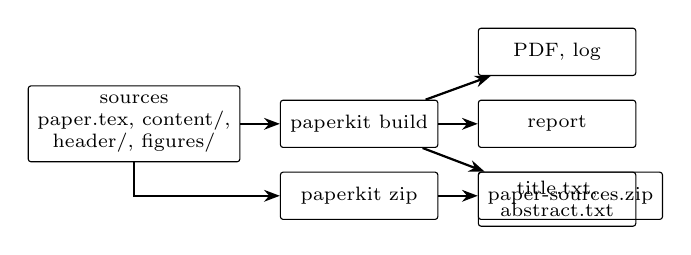
\begin{tikzpicture}[
    node distance=3mm and 5mm,
    box/.style={draw, rounded corners=1pt, minimum width=20mm, minimum height=6mm,
      font=\scriptsize, align=center},
    arr/.style={-{Stealth[length=2mm]}, thick},
  ]
  \node[box] (src) {sources\\paper.tex, content/,\\header/, figures/};
  \node[box, right=of src] (build) {paperkit build};
  \node[box, above right=of build] (pdf) {PDF, log};
  \node[box, right=of build] (report) {report};
  \node[box, below right=of build] (txt) {title.txt,\\abstract.txt};
  \node[box, below=of build] (zip) {paperkit zip};
  \node[box, right=of zip] (archive) {paper-sources.zip};
  \draw[arr] (src) -- (build);
  \draw[arr] (build) -- (pdf);
  \draw[arr] (build) -- (report);
  \draw[arr] (build) -- (txt);
  \draw[arr] (src) |- (zip);
  \draw[arr] (zip) -- (archive);
\end{tikzpicture}

  % acmart requires a \Description for every figure, for screen readers, and
  % warns about each one that lacks it.
  \Description{Sources on the left feed paperkit build, which produces the
  PDF, the report and the text exports; paperkit zip produces the archive.}
  \caption{One build produces the PDF, the build log, the exported title and
  abstract, and the report; one \texttt{paperkit zip} produces the archive.
  Nothing on the right is committed.}
  \label{fig:overview}
\end{figure}

\paragraph{Sources in directories}
The main file \texttt{paper.tex} names the pieces and their order; the text
lives in \texttt{content/}, numbered so that the directory listing reads like
the table of contents, and the preamble in \texttt{header/}.
Figure~\ref{fig:overview} is itself a \TeX\ source, kept with the other
figures, so it is typeset with the paper's fonts and needs no conversion.

\paragraph{Two targets}
The supplementary material is a second main file in the same tree. It shares
\texttt{header/} and the bibliography, so a macro renamed in one place is
renamed in both, and an entry cited only in the appendix is not reported as
unused when the paper is checked.

\paragraph{A pinned environment}
The configuration names a dated \TeX\ Live snapshot and its checksum, so the
image that builds the paper has the same packages on every rebuild, on every
machine, and the build timestamp comes from the commit, so two builds of one
commit produce the same bytes~\cite{reproducible}.

\section{Evaluation}
\label{sec:evaluation}

Table~\ref{tab:checks} lists what the report says for this project. Each row
is a check that paperkit runs after the build, and each one has a reason to
exist: the fonts row is what ACM's TAPS rejects first, the page row is what
the chairs count, and the bibliography rows are what reviewers notice.

\begin{table}[t]
  \caption{The report for this example. A real paper reads the same table
  after every build.}
  \label{tab:checks}
  \begin{tabular}{ll}
    \toprule
    Check & Result \\
    \midrule
    LaTeX errors and warnings & none \\
    Overfull and underfull boxes & none \\
    Fonts & all embedded, no Type 3 \\
    Non-ASCII, whitespace, newline & clean \\
    Unused bibliography entries & none \\
    bibtex-tidy & tidy \\
    Pages before the references & 1 of 12 \\
    \bottomrule
  \end{tabular}
\end{table}

The one check this layout makes interesting is the unused-entry check. The
bibliography serves both targets, so paperkit gathers the citations of each
from its build output before deciding that an entry is unused, and an entry
the appendix cites~\cite{tlnet} is in use even though this paper never cites
it. The full tables are in the supplementary material.

\section{Conclusion}

A paper project has a shape that makes it easy to check, and this example is
that shape: sources in directories, one configuration file that says how the
paper is built and what it must satisfy, and nothing generated under version
control. Copy it, rename the main files, and replace the text.


\begin{acks}
% ACM calls state the page limit as "N pages, not including references", so
% these acknowledgments count toward the budget; the acm profile tells
% paperkit as much (ack_counts_as_content).
This example was written for paperkit's users. Funding lines, grant numbers
and the names of the reviewers go here.

\end{acks}

\bibliographystyle{ACM-Reference-Format}
\bibliography{content/references}

\end{document}
